What is the relationship between a Transnational Entrepreneur's
network and their knowledge diffusion within the context of the Berlin
Startup sphere.

\section{Literature Review}
Transnational Entrepreneurs are conceptualized as individuals embedded
in wider cross-border business networks and socio-political
institutions that shape the attitudes and behaviors of individual
entrepreneurs. Formally, they are defined as ``individuals who migrate
from one country to another, concurrently maintaining business-related
linkages with their countries of origin and current adopted countries
and communities'' \cite{Drori.2009}.

A simplified example of this phenomenon may be explained as follows.
Imagine that you have an individual from ``Country A''. This
individual grows up in ``Country A'' and develops a network within
their home country. This individual then migrates to ``Country
B''. Within ``Country B'' they develop a new network of individuals
composed of people from ``Country B''. The role of this special
individual is to now serve as a bridge between ``Country A'' and
``Country B''. This paper seeks to explore the nature of the
individual as a bridge and how they affect the development of economic
activities within the entrepreneurial space.

Transnationalism can be an important economic driver in the
development of new businesses and new technologies. As an example, in
transnational activities between New Zealand and South Korea,
``economic activities that have developed as a result''
\cite{Collins.2008}. In another example, the value of Transnationalism
socio-economic activities is more clearly delineated ``In addition,
transnational economic resources can be transformed into local social
resources or vice versa, as well as transnational social resources,
which can transform into local economic resources or vice versa''
\cite{Ren.2015}.

This paper seeks to study transnational entrepreneur networks within a
digital context, because ``Although networks have been considered
crucial to transnational entrepreneurship (TE), there has been a lack
of theoretical and methodological engagement with social network
analysis in the existing TE research''\cite{Chen.2009}.

The reason why it is so important to understand the network and how it
moderates transnational entrepreneurial activities is because it is
the basis of what defines a transnational entrepreneur, yet it is
poorly understood.

\section{The Theoretical Model}
The theoretical model dictates that knowledge diffusion within a
Transnational Entrepreneur's network is moderated by their network
distribution. Below, we will summarize the premises necessary to come
to this conclusion and how we will systematically build our logic to
this testable hypothesis.

\begin{figure}[!ht]
  \centering
  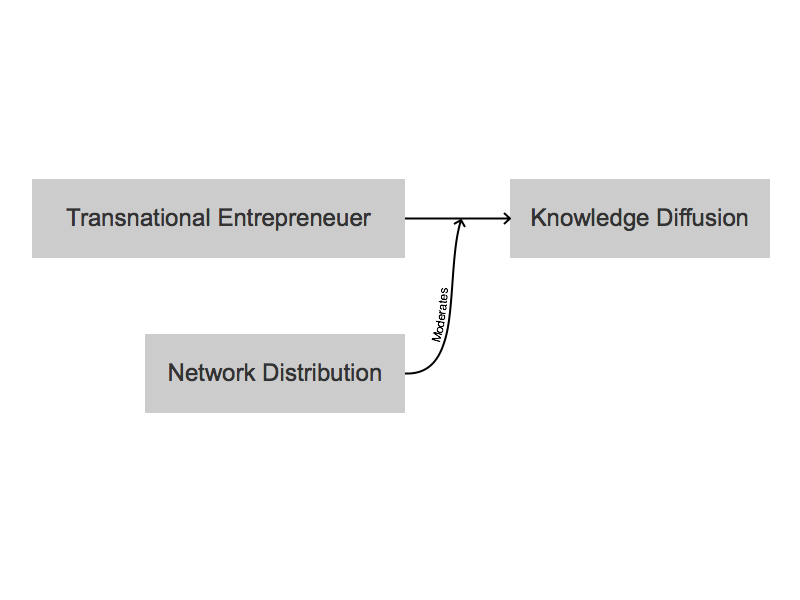
\includegraphics[width=1.0\textwidth]{theoretical_model.png}
  \caption{Knowledge Diffusion is moderated by Network Distribution.}
\end{figure}

\subsection{Premises: Transnational Entrepreneur}
There exist a set of individuals that fit the criteria of a
Transnational Entrepreneur. The criteria state that a Transnational
Entrepreneur is an entrepreneur which leverages two or more distinct
national networks in their business operations.

Furthermore, the hypothesis postulates that Transnational
Entrepreneurs diffuse knowledge across national borders.

Finally, it can be said that the frequency of knowledge diffusion
across borders within a Transnational Entrepreneur's network is
moderated by their network's nationality distribution. The national
distribution refers to the relative populations of different
populations as constrained by socio-ethnic groups. That is, with
different distributions, occur different rates of transnational
diffusion.

\section{Hypothesis}
Network Distribution Normalization \& Transnational Diffusion are
positively Correlated. The closer the Transnational Entrepreneur's
network demographics are to a normalized distribution, the higher the
frequency of transnational diffusion. A normalized distribution is
defined within a statistical context. This means that 32\% of a user's
network should fall within one distribution, another 32\% within
another. Following this same reasoning, 95\% of a given Transnational
Entrepreneur's network should fall within four discrete countries.
\begin{figure}[H]
  \centering
  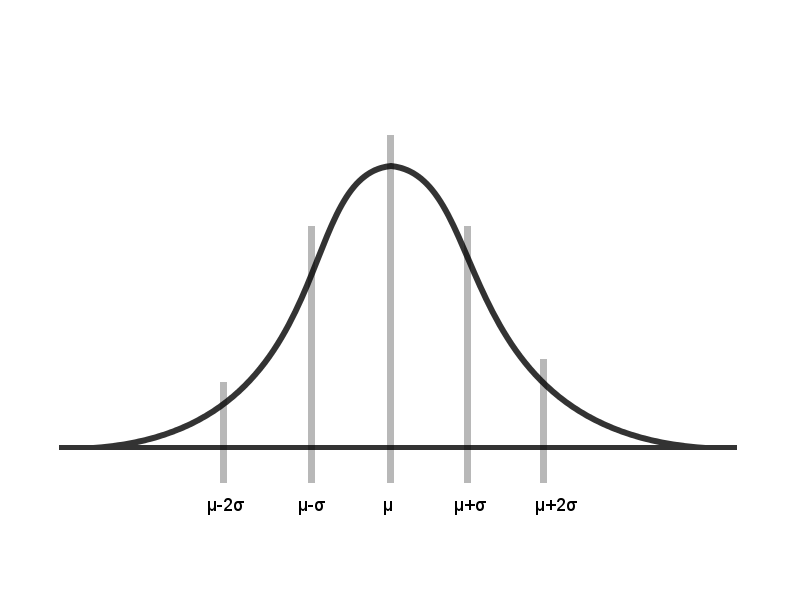
\includegraphics[width=1.0\textwidth]{normal_distribution.png}
  \caption{Normalized distribution (not drawn to scale).}
\end{figure}

In order to measure the deviation from a normal distribution, we will
measure the Kurtosis. Kurtosis is a measure of the ``tailedness'' of a
probability distribution. Kurtosis can be characterized in three ways:
mesokurtic, leptokurtic, and platykurtic. A most normal distribution
is mesokurtic. A leptokurtic distribution is one that is very peaky,
it has a tall center, and platykurtic distribution is one that is very
wide, and evenly distributed. Our hypothesis is, therefore, there
exists a relationship between the delta of a mesokurtic distribution
and the frequency of transnational diffusion in a given network.
